
\documentclass[11pt]{article}

\usepackage{common}
\usepackage{listings}
\usepackage[toc,page]{appendix}
\title{HW4: Word Segmentation}
\author{Virgile Audi \\ vaudi@g.harvard.edu \\ Nicolas Drizard \\ nicolasdrizard@g.harvard.edu}
\begin{document}

\maketitle{}
\section{Introduction}

The goal of this assignement is to tackle the NLP task of identifying and labeling contiguous segments of text. We will use sequence models and a dynamic programming method to find the best scoring sequence.


\section{Problem Description}

The idea is here to label continuous sequence of words with BIO tagging of different entities. The entities are the following:

\begin{enumerate}
	\item PER: a person
	\item LOC: a location
	\item ORG: an organization
	\item MISC:
\end{enumerate}

Furthermore, this tagging method identifies the continuous group of words belonging to the same entity: the prefix B stop the current tag and begins a new one whereas the prefix I continues adding to the previous tag. However, in our solution we just cared about predicting the entity tag and then we were grouping the contiguous predictions into the same entity because the training text does not contain any B-tag.


\section{Model and Algorithms}

We used three different methods to solve this problem. The first two are the equivalent of first the Naive Bayes and second the logistic regression from text classification tasks. The last one introduces a customized way to train a neural architecture for this task.

\subsection{Hidden Markov Model}

We implement here a standard first order hidden Markov Model. The hidden states are the tags and the observed states are the features we built (word counts, capitalization...). The model can be represented with the following graphical model and requires two distribution: emission and transition.

\begin{figure}[H]
\begin{center}
    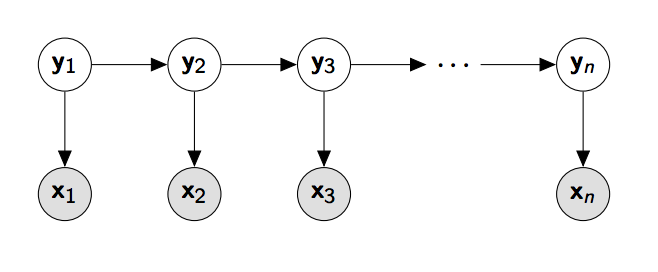
\includegraphics[width=0.5\textwidth]{hmm}
    \caption{Graphical model of 1st order HMM with one feature}
\end{center}
\end{figure}

We represent the two distrubitions with multinomial as they model feature counts. As a result, we can infer them simply with the maximum likelihood estimator:

\[
p(x_i=\delta(f)|y_i=\delta(c)) = \frac{F_{f,c}}{F_{.,c}}
\]
\[
p(y_i=\delta(c_i)|y_{i-1}=\delta(c_{i-1})) = \frac{T_{c_{i-1},c_i}}{T_{c_{i-1},.}}
\]

with $T_{c_{i-1},c_i}$ the counts of class $c_{i-1}$ preceding class $c_i$ and $F_{f,c}$ the counts of emission f with class c.

If we consider multiple features, then we still assume that the feature are indepent with each other (it's the main assumption in the Naive Bayes approach also). Only the emission distribution is changed and we can combine the probability together:

\[
p(x_i=(\delta(f_1), \delta(f_2))|y_i=\delta(c)) = p(x_i=\delta(f_1)|y_i=\delta(c)) p(x_i=\delta(f_2)|y_i=\delta(c)) =
\frac{F_{f_1,c}}{F_{.,c}}  \frac{F_{f_2,c}}{F_{.,c}}
\]




\subsection{Maximum-Entropy Markov Model}

Next, we implemented a Maximum-Entropy Markov Model. The objective of the MEMM is to evaluate at each time step a distribution over the possible tags using features of the current word, denoted as $feat(x_i)$ and the tag of the previous word, $c_{i-1}$, using multi-class logistic regression, i.e.

$$p(\mathbf{y}_i | \mathbf{y}_{i-1}, feat(x_i)) = \text{softmax}([feat(x_i),c_{i-1}]\mathbf{W}+\mathbf{b})$$

\subsection{Viterbi algorithm}

The search algorithm that we implemented is the dynamic programming algorithm named after Andrew Viterbi. Its main difference with a greedy approach is that it evaluates at every step and for every previous state, the best possible next step. This guarantees a solution closer to the true optimal solution. The pseudo-code of the algorithm is given by:\\

\begin{algorithmic}
    \Procedure{ViterbiWithBP}{}
    \State{$\pi \in \reals^{ n+1 \times \mcC}$ initialized to $-\infty$ }
    \State{$bp \in \mcC^{n \times \mcC}$ initialized to $\epsilon$ }
    \State{$\pi[0, \langle s \rangle] = 0$}
    \For{$i = 1$ to $n$ }
    \For{$c_{i-1} \in \mcC$}
    \State{compute $\hat{\boldy}(c_{i-1})$}
    \For{$c_{i} \in \mcC$}
    \State{$score = \pi[i-1, c_{i-1}] + \log \hat{\boldy}(c_{i-1})_{c_i} $}
    \If{$score > \pi[i, c_i]$}
    \State{$\pi[i, c_i] = score$}
    \State{$bp[i, c_i] = c_{i-1}$}
    \EndIf{}
    \EndFor{}
    \EndFor{}
    \EndFor{}
    \State{\Return{sequence from $bp$}}
    \EndProcedure{}
  \end{algorithmic}

\subsection{Structured Perceptron}

The final model, we implemented is the structure perceptron train algorithm. The way the model is trained uses the Viterbi search algorithm, presented above. At each epoch, we uses Viterbi to predict the highest scored sequence given the state of the model. We can then find the timesteps where the actual sequence for the given sentence and the predicted one differ and compute at each of these time steps, the gradient of a hinge type loss. These gradients have a -1 entry on the true class for this given word, and a 1 on the predicted class by the model. We can then propagate these gradients in the network, and update the weights with a learning rate that can be tuned.\\

The model itself is similar to the model of the MEMM without the final logsoftmax layer.
\section{Experiments}

\subsection{Feature Engineering}

The original paper suggests several features to use. We focus on the word counts and a capitalization feature. We defined our capitalization feature as follow:
\begin{enumerate}
	\item 1 : word in low caps;
	\item 2 : whole word in caps;
	\item 3 : first letter in cap;
	\item 4 : one cap in the word;
	\item 5 : other
\end{enumerate}

We then produced an embedding of the word counts using a pre-trained version.\\

We also used the Python "pattern.en" package to extract Part-of-Speach (PoS) features. The packages generates 41 features to which we added special feature for the opening and closing tabs $<$s$>$ and $<\setminus$s$>$.


\subsection{Model Evaluation}

As used in the Kaggle competition, we used the f-score with the precision and recall measure to evaluate our model while tuning the hyperparameters. A positive prediction stands for a label (in the notation of the task, everything which is not the \textbf{O} tag):

\begin{enumerate}
	\item recall: ratio of the true positive predictions among the positives tags in the correct sequence
	\item precision: ratio of the true positive predictions among the positive predictions,
	\item f-score (with $\beta = 1$): harmonic mean of the precision and the recall, i.e. $f_{1} = \frac{2pr}{p+r}$
\end{enumerate}

\subsection{Hidden Markov Model}

There is only the smoothing parameter $\alpha$ and eventually feature selection here to tune here. We evaluate the impact of adding more features and run experiments with different alpha values to tune them . One important details is to make sure to use a specific smoothing parameter for each distribution, i.e a smoothing parameter may be applied to the transition matrix but also to the emission matricx of each different feature. Each of this distribution has a different tail and need a different smoothing. For instance, the transition matrix need a very small $\alpha$ (around 0.1) because we are pretty confident in it but the capitalizations feature need one much bigger (around 20) because the counts are already high.

\begin{figure}[H]
\centering
\begin{minipage}{.5\textwidth}
  \centering
  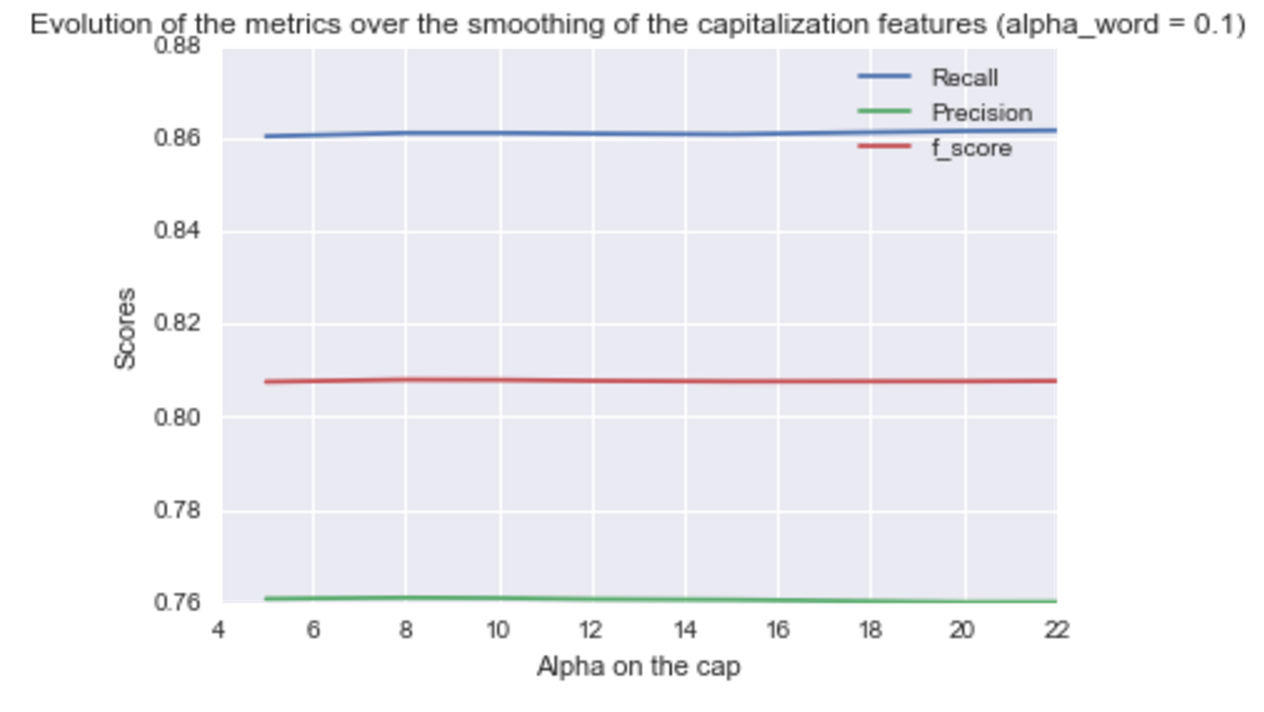
\includegraphics[width=1\linewidth]{cap_plot}
\end{minipage}%
\begin{minipage}{.5\textwidth}
  \centering
  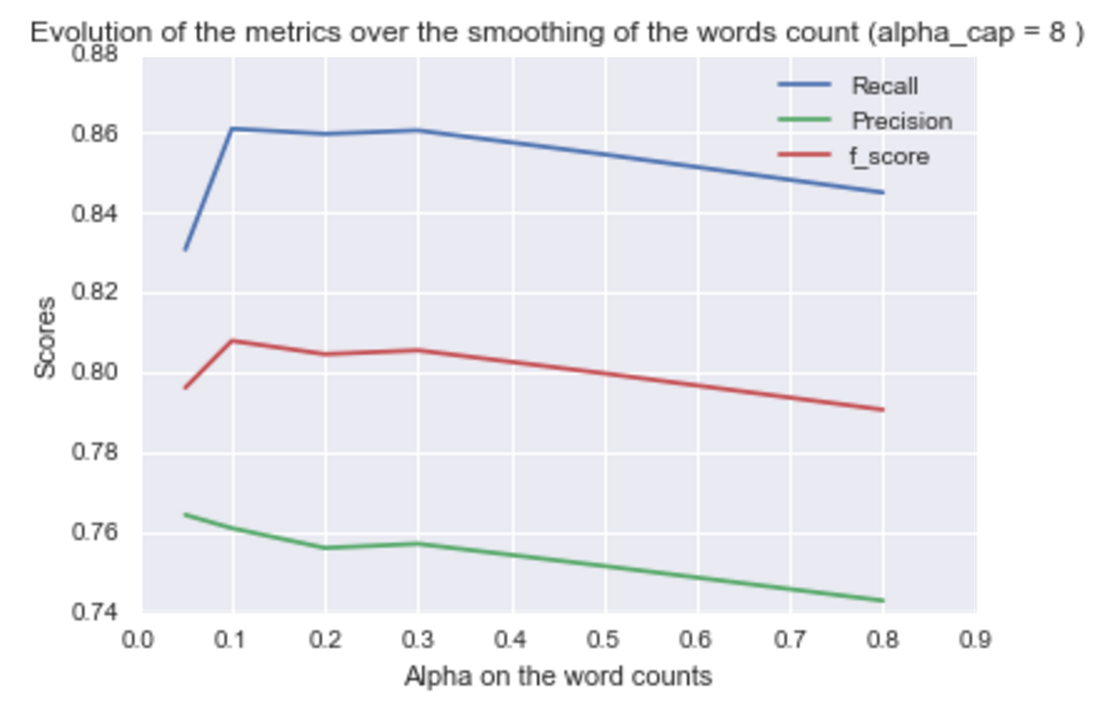
\includegraphics[width=1\linewidth]{wc_plot}
\end{minipage}
\end{figure}

We notice that the model is less sensitive to the changes of the smoothing parameter on the capitalization feature as on the word counts. This is pretty reasonable as the feature coutns are much higher in the capitalization feature than in the word counts. Tuning this parameter provides a model with a f-score of \textbf{0.808}. Using only the word counts features provide a best f-score of \textbf{0.764}.\\

We obtained a Kaggle score on the test set of :

$$K_{HMM} = 0.48365$$

\subsection{Maximum-Entropy Markov Model}

We coded the MEMM using the nn module and trained using stochastic gradient descent. We also used the Glove embedggins using a lookup table. As for the HMM, we used two different sets of features, i.e. the words and the words and capitalisation of the words. We also added the Part of Speech features that were evaluated using the python package "pattern.en" in order to gain some time. We observed that the training algorithm converges quite rapidely, and that if adding caps to the features helped decrease the loss, the impact was not as strong as expected. On the other hand, adding PoS features impacted greatly the loss. Nevertheless, we trained the model on 20 epochs in order to learn the embeddings for the $<$s$>$ and $<\setminus$s$>$ "words" added during pre-processing.

\begin{figure}[H]
\centering
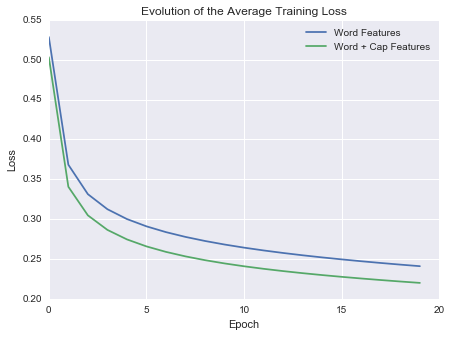
\includegraphics[width=0.6\linewidth]{loss_mem}
\end{figure}

We evaluated the performance of these two models using the f-score presented above:

\begin{figure}[H]
\centering
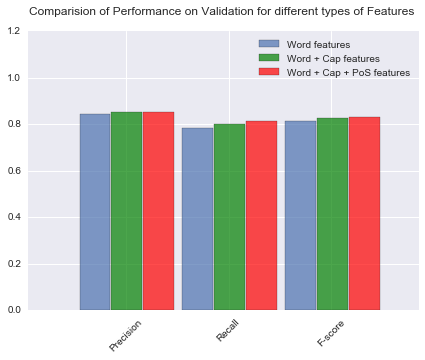
\includegraphics[width=0.6\linewidth]{prf_cap}
\end{figure}

Adding extra features yielded better results on both Precision and Recall and therefore on the f-score. But as we expected from the small differences in loss, we did not observe an important increase on the f-score using cap features. We were nevertheless surprised to see that the impact on loss using PoS features did not translate on the f-score. These results were later confirmed on the test set, as the kaggle score obtained for these two models were:

$$K_{no caps} = 0.52057 \quad \text{and} \quad K_{caps} = 0.55482 \quad K_{PoS} = 0.57121$$

which are both slightly better than the results of the HMM.

\subsection{Structured Perceptron}


\section{Conclusion}

This segmentation task gave us the opportunity to implement different recurrent neural network architectures but also to compare them with more traditionnal method. Whereas the count based and even the simple neural network models are pretty fast to train they still provide interesting results. The results provided by the three variants of RNN were interesting to illustrate the influence of gates and memory in such networks. The gated reccurent network ended as the best model on this task. One future work could be to stack more layers to our reccurent architecture or to implement a network with a dynamic memory part to give more flexibility in how the model uses the information it already processed.



\begin{appendices}
\textbf{\huge\underline{Preprocessing:}}
\lstinputlisting[numbers=left, breaklines=true]{../preprocess.py}

\textbf{\huge\underline{Hidden Markov Model:}}
\lstinputlisting[numbers=left, breaklines=true]{../hmm.lua}

\textbf{\huge\underline{Max-Entropy Markov Model:}}
\lstinputlisting[numbers=left, breaklines=true]{../MEMM.lua}

\textbf{\huge\underline{Helper:}}
\lstinputlisting[numbers=left, breaklines=true]{../helper.lua}
\end{appendices}
\end{document}
